\documentclass[a4paper,12pt,oneside]{article}

% Imported packages
\usepackage[english]{babel}
\usepackage[T1]{fontenc}
\usepackage[utf8]{inputenc}
\usepackage{amssymb}
\usepackage{amsmath}
\usepackage{bm}
\usepackage{listings}
\usepackage{graphicx}
\usepackage{geometry}
\usepackage{float}
\usepackage{subfig}
\usepackage{wrapfig}
\usepackage{color}
\usepackage{comment}
\usepackage{hyperref}
\usepackage{bigfoot} % to allow verbatim in footnote
\usepackage{bigfoot} % to allow verbatim in footnote
\usepackage[numbered,framed]{matlab-prettifier}
\usepackage{filecontents}

\let\ph\mlplaceholder % shorter macro
\lstMakeShortInline"

\lstset{
  style              = Matlab-editor,
  basicstyle         = \mlttfamily,
  escapechar         = ",
  mlshowsectionrules = true,
}

% Margin dimensions settings
\geometry{a4paper,top=2cm,bottom=2cm,left=2cm,right=2cm,
	heightrounded,bindingoffset=5mm}

% Enumeration settings
\renewcommand{\thesection}{\arabic{section})}
\renewcommand{\thesubsection}{\arabic{section}\alph{subsection})}

% x bar for UTF-8 encoding
\DeclareUnicodeCharacter{304}{$ \bar{x} $}

% Code visualization settings
\lstset{basicstyle=\small\ttfamily}

% Code design settings
\lstset{language=Matlab}

% Included images path
\graphicspath{{Images/}}

% Document information
\title{Fundamentals of Vibration Analysis and Vibroacoustics \\
	Module 2 - Vibroacoustics of Musical Instruments \\
	Assignment 2 - Experimental modal analysis of a violin}
\author{Bombaci Nicola 10677942 \\
	Fantin Jacopo 10591775 \\
	Intagliata Emanuele 10544878}
\date{June 2020}


\begin{document}

\maketitle

\vspace{100pt}


\section{\textsc{Matlab} code for modes identification}

Starting from the experimental data collected into \lstinline!Data.mat! file we implemented the \textsc{Matlab} script for identifying the modes according to the
procedure described in laboratory slides.

\subsection{Minimization algorithm}

In order to study the vibrational modes of the violin starting from these experimental data, we refer to the \textbf{modal approach}, that describes the overall frequency response of a structure as superposition of $ N $ modes of vibration, as far as enough modes are considered:

\begin{equation}
\label{eqn:h_exp_modal} 
	G^\textup{EXP}_{jk}(\omega) \approx \sum_{i=1}^{N} \frac{X_j^{(i)} X_k^{(i)} / m_i}
		{-\omega^2 + j 2 \omega_i \omega \xi_i + \omega^2_i}
		\text{~ , ~}
		\xi_i = \frac{c_i}{2 m_i \omega_i}
\end{equation}

For well distinguished peaks and lightly damped structures, the FRF $ G_{jk} (\omega) $ can be approximated around a certain $ \omega_i $ as:

\begin{equation}
\label{eqn:h_approx} 
	G^\textup{NUM}_{jk}(\omega) \approx \sum_{i=1}^{N} \frac{ A_{jk}^{(i)} }
		{-\omega^2 + j 2 \omega_i \omega \xi_i + \omega^2_i}
		+ R^H_{jk} + \frac{R^L_{jk}}{\omega^2}
		\text{~ , ~}
		\omega_\textup{inf} < \omega_i < \omega_\textup{sup}
\end{equation}

\begin{figure}[H]
	\centering
	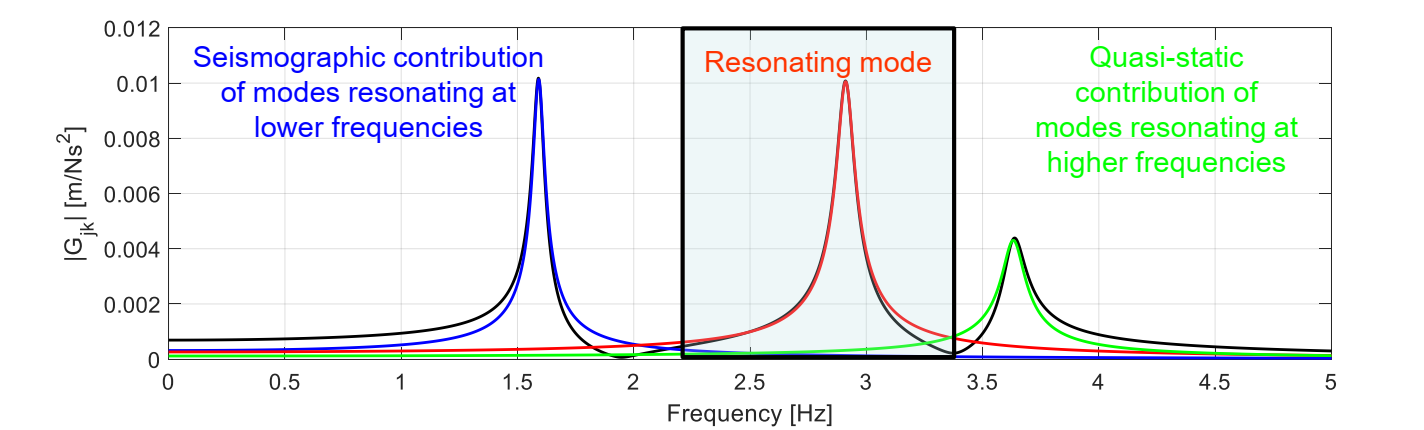
\includegraphics[scale=0.5]{Gapprox_slides}
\end{figure}

The first thing we had to implement was an algorithm in order to find the frequency ranges of interest. We decided to divide the frequency axis in $ N $ partitions (where $ N $ is the number of identified peaks or considered modes).

Given the $ N $ peaks found (i.e. $ N $ maxima, see \ref{peak_search} ) we found $ N + 1 $ minima between those peaks (and the endpoints of the frequency axis).

\begin{lstlisting}[caption = {Frequency range search}]
	wp_dx = iini;
	for yy = 1: (Nmodes + 1) % over the m(+1) peaks
		wp_sx = wp_dx; % left end is former right end
    
	if yy > Nmodes % right end
		wp_dx = i_max;
	else
		wp_dx = indices(yy); % frequency of next peak (right end)
	end
	[~, min_index] = min(abs(FRF_LP(wp_sx:wp_dx, :)), [], 1);
	rfi(:,yy) = min_index + wp_sx - 1;
end
\end{lstlisting}

We obtain a set of $ N + 1 $ values of $ \omega $
(i.e. the endpoints of the frequency ranges) for each measurement.

This is maybe not the most precise way to deal with this kind of problem but it can be seen in the last section that good results are delivered.

For a given set of experimental FRFs $ G^{EXP} $, obtained for a fixed measurement location $ j $ and different excitation locations $ k $ (grid of points), a \textbf{least squares minimization procedure} can be implemented for the estimation of the \textbf{modal parameters} $ (X^{(i)}, \omega_i, \xi_i, m_i) $.

Considering the experimental FRF matrix $ \mathbf{G^\textup{EXP}} $, it shows:

\begin{list}{}
	\item a number $ m $ of rows corresponding to the length of the frequency vector $ \omega $;
	\item a number $ n $ of columns corresponding to the $ k - j $ pairs (i.e. the available FRFs).
\end{list}

Here we have that:

\begin{list}{}
	\item $ G_r^\textup{EXP} (\omega_s) $ is a generic element of the experimental FRF matrix $ \mathbf{G^\textup{EXP}} $ corresponding to the $ r $-th column (FRF) evaluated in correspondence of the frequency $ \omega_s $;
	\item $ G_r^\textup{NUM} (\omega_s) $ is the numerical FRF estimation around a certain $ \omega_i $, corresponding to the $ r $-th column (FRF) evaluated in correspondence of the frequency $ \omega_s $, i.e.

		\[
			G^\textup{NUM}_k(\omega_s) = \sum_{i=1}^{N} \frac{ A_{r}^{(i)} }
				{-\omega_s^2 + j 2 \omega_i \omega_s \xi_i + \omega^2_i}
				+ R^H_{r} + \frac{R^L_{r}}{\omega_s^2}
		\]
\end{list}

\subsection{Error minimization problem}

The \textbf{error function} to be minimized should then be:
\begin{equation}
\label{eqn:error_fun} 
	\varepsilon = 
		\sum_{r=1}^{N}
		\sum_{s=s_\textup{inf}}^{s_\textup{sup}}
		\Re^2\{G^\textup{EXP}_r(\omega_s) - G^\textup{NUM}_r(\omega_s)\} +
		\Im^2\{G^\textup{EXP}_r(\omega_s) - G^\textup{NUM}_r(\omega_s)\}
\end{equation}

Since the error function depends non-linearly from the unknown parameters, an \textsl{iterative} minimization procedure must be used.

For an iterative procedure an \textbf{initial guess vector} $ x_0 $ is required, consisting of a preliminary estimate of:

\begin{list}{}
	\item $ \omega_i $  which is found from the maximum peak in the considered frequency range (see section \ref{peak_search};
	\item $ \xi_i $ which is found through some simplified method, assuming that just the
resonating mode is contributing to the system response. We used the \textbf{phase derivative method}:
		\[
			\xi_i = - \frac{1}{\omega_i \frac{\partial \angle G_{jk}}{\partial \omega}\big|_{\omega =
				\omega_i}}
		\]
 
	\item $ A_r^{(i)} $ which is found considering each FRF at resonance and assuming real valued mode shapes:
\[
	A_r^{(i)} \approx - \Im (2 \xi_i \omega_i^2 G_r^\textup{EXP}(\omega_i))
\]
	\item $ R_r^L $ and $ R_r^R $ are set to zero under the assumption of sufficiently distinguished peaks.
\end{list}

It can be seen that the non-linear minimization procedure elaborates \textsl{simultaneously} the whole set of FRFs, leading to an estimate of $ \omega_i, \xi_i, A^{(i)}_r $.
This is not a trivial problem from a computational point of view.

Firstly we tried to implement this procedure using \lstinline!fminsearch! function. It finds the minimum of unconstrained multivariable function using derivative-free method. It is a nonlinear programming solver and searches for the minimum of a problem specified by

\[
	\min_x f(x)
\]

where \lstinline!f(x)! is a function that returns a scalar, and \lstinline!x! is a vector or a matrix. 

In our case \lstinline!x! is a set of modal parameters vectors (one for each measurement) and \lstinline!f(x)! should be the error function seen in eq. (\ref{eqn:error_fun}).

This approach led to a runtime of almost an hour.

In our second attempt we used the \textsc{Matlab} function \lstinline!lsqnonlin! (as suggested in laboratory slides). This function solves a non-linear least-squares curve fitting problem of the form:

\[
	\min_x ||f(x)||_2^2 =
	\min_x \left(f_1 (x)^2 + f_2(x)^2 + \ldots + f_n (x)^2 \right) 
\]

Rather than computing the value $ ||f(x)||_2^2 $ (the sum of squares), \lstinline!lsqnonlin! requires the user-defined function to compute the \textit{vector-valued} function:

\[
	f(x) = 
		\begin{bmatrix} f_1 (x) \\ f_2 (x) \\ \vdots \\ f_n (x) \end{bmatrix}
\]

In other words, \lstinline!x = lsqnonlin(fun, x0)! starts at the point \lstinline!lsqnonlin(fun,x0)! and finds a minimum of the sum of squares of the functions described in \lstinline!fun!. The function \lstinline!fun! should return a vector (or array) of values and not the sum of squares of the values. The algorithm implicitly computes the sum of squares of the components of \lstinline!fun(x)!.

This function forces us to use a slightly simplified version of the \textbf{error function}:
\begin{equation}
\label{eqn:error_fun2} 
	\varepsilon = \sum_{s=s_\textup{inf}}^{s_\textup{sup}}
		\Re^2\{G^\textup{EXP}(\omega_s) - G^\textup{NUM}(\omega_s)\} +
		\Im^2\{G^\textup{EXP}(\omega_s) - G^\textup{NUM}(\omega_s)\}
\end{equation}

In this way the non-linear minimization procedure elaborates the FRFs \textsl{one-by-one}.

This leads us to a less precise minimization algorithm. On the other hand now it is much faster. 

Using \lstinline!lsqnonlin! we provide a \lstinline!f(x)! of this form:

\[
	f(x) = 
		\begin{bmatrix}
			f_1 (x) \\
			f_2 (x)
		\end{bmatrix} =		\begin{bmatrix} 
										\Re\{G^\textup{exp}(\omega_s) - G^\textup{num}(\omega_s)\} \\
										\Im\{G^\textup{exp}(\omega_s) - G^\textup{num}(\omega_s)\}  
									\end{bmatrix}
\]

Remember: the algorithm implicitly computes the sum of squares of the components of \lstinline!f(x)!.

\begin{lstlisting}[caption = {Snippet of code from \texttt{err\_i.m}}]
	% error computation
	c_e = H_exp - H_num; %complex error
	real_e = (real(c_e));
	imag_e = (imag(c_e));
	error = [real_e; imag_e];
\end{lstlisting}

In the end the minimization process gives us an estimation of the modal parameters $ \xi_i, \omega_i, X^{(i)}, R_r^L $ and $ R_r^R $.

Setting $ m_i = X_r^{(i)} $, the normalized mode shape at each of the $ k $ locations is given by the gain $ A_r^{(i)} = X_r^{(i)} $
Other useful modal parameters can be found in function of the previous ones:

\begin{gather*}
	c_i = 2 m_i \omega_i \xi_i \\
	k_i = \omega_i^2 m_i
\end{gather*}

\subsection{FRF Reconstruction}
The FRFs are reconstructed using the custom function \lstinline!reco.m!. It takes as input a vector with modal parameters and gives as output the reconstructed FRF, using the formulation seen in eq. (\ref{eqn:h_exp_modal}).

\begin{lstlisting}[caption = {Snippet of code from \texttt{reco.m}}]
	for mm = 1:meas
		for pp = 1:nPeaks
			FRF_reco(:, mm) = FRF_reco(: , mm) + ...
				(Aj(pp,mm) + 1i*Bj(pp,mm))./(- m_i(pp,mm).*omega.^2 + 1i*c_i(pp,mm).*omega +
				k_i(pp,mm));
		end
	end
\end{lstlisting}

Quality of the estimates can be visually assessed comparing in a plot the
identified FRFs $ G^\textup{NUM} $ with the experimental ones $ G^\textup{EXP} $ . We will see it in the next sections.

\section{Software testing}

\subsection{Data pre-processing}

The given \lstinline!Data.mat! file contains experimental FRFs $ [m / s^2 N] $ that have been obtained performing a hammer test on a violin, following a roving hammer procedure, that consists in fixing the measurement position(s) while varying excitation location.
The coordinates of the measuring grid can be found in the variable \lstinline!xy!. The measuring grid is reported in the figure below.

\begin{figure}[H]
	\centering
	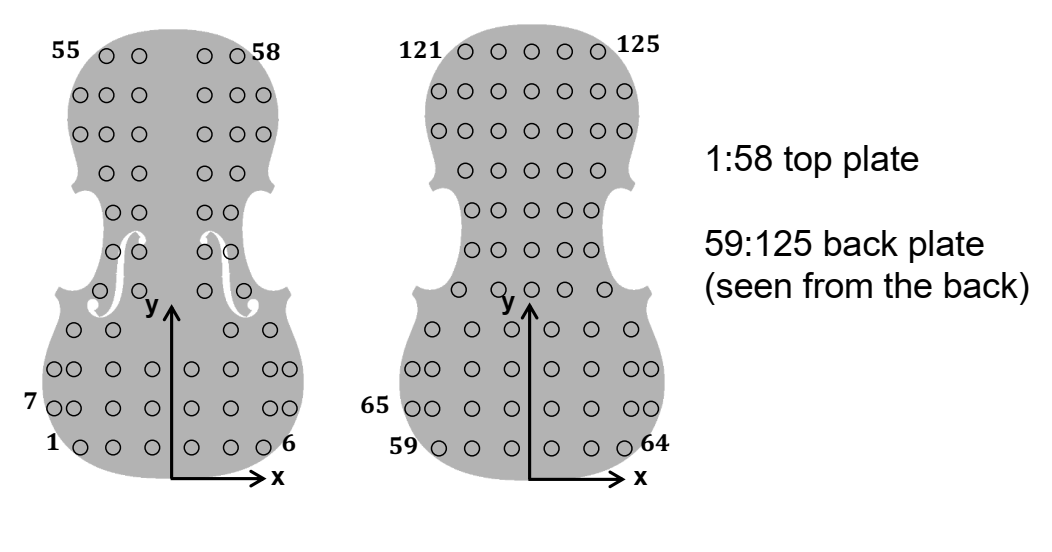
\includegraphics[scale=0.4]{grid_slides}
\end{figure}

To sum up, \lstinline!Data.mat! contains the frequency vector (\lstinline!freq!), the experimental FRF matrix (\lstinline!FRF!, measurement direction positive outward with respect to the top plate), the measurement grid (\lstinline!xy!), the contours of front plate (\lstinline!xy_bt!) and back plate (\lstinline!xy_bf!).

First of all we converted the unit of measurement of the FRFs from an acceleration over a force $ [m / s^2 N] $ to a displacement over a force $ [m / N] $. To do so we divided the FRFs by the vector $ \omega^2 $ using the function \lstinline!repmat!.

Being the frequency response spectra very noisy, we decided to smooth them out, extracting only the envelope.

\subsection{Peak search}
\label{peak_search} 

The steps we followed to identify the resonance frequencies, which correspond to the relative maxima of the module diagram of the FRFs:

\begin{itemize}
	\item Computing the mean FRF over all the low-passed FRFs, considering those measured for points on the front plate together with those for points on the back plate, and we low-passed again the result. This way, we would be quite sure to identify vibration modes in common between the two plates.

		\begin{figure}[H]
			\hspace{-70pt}
			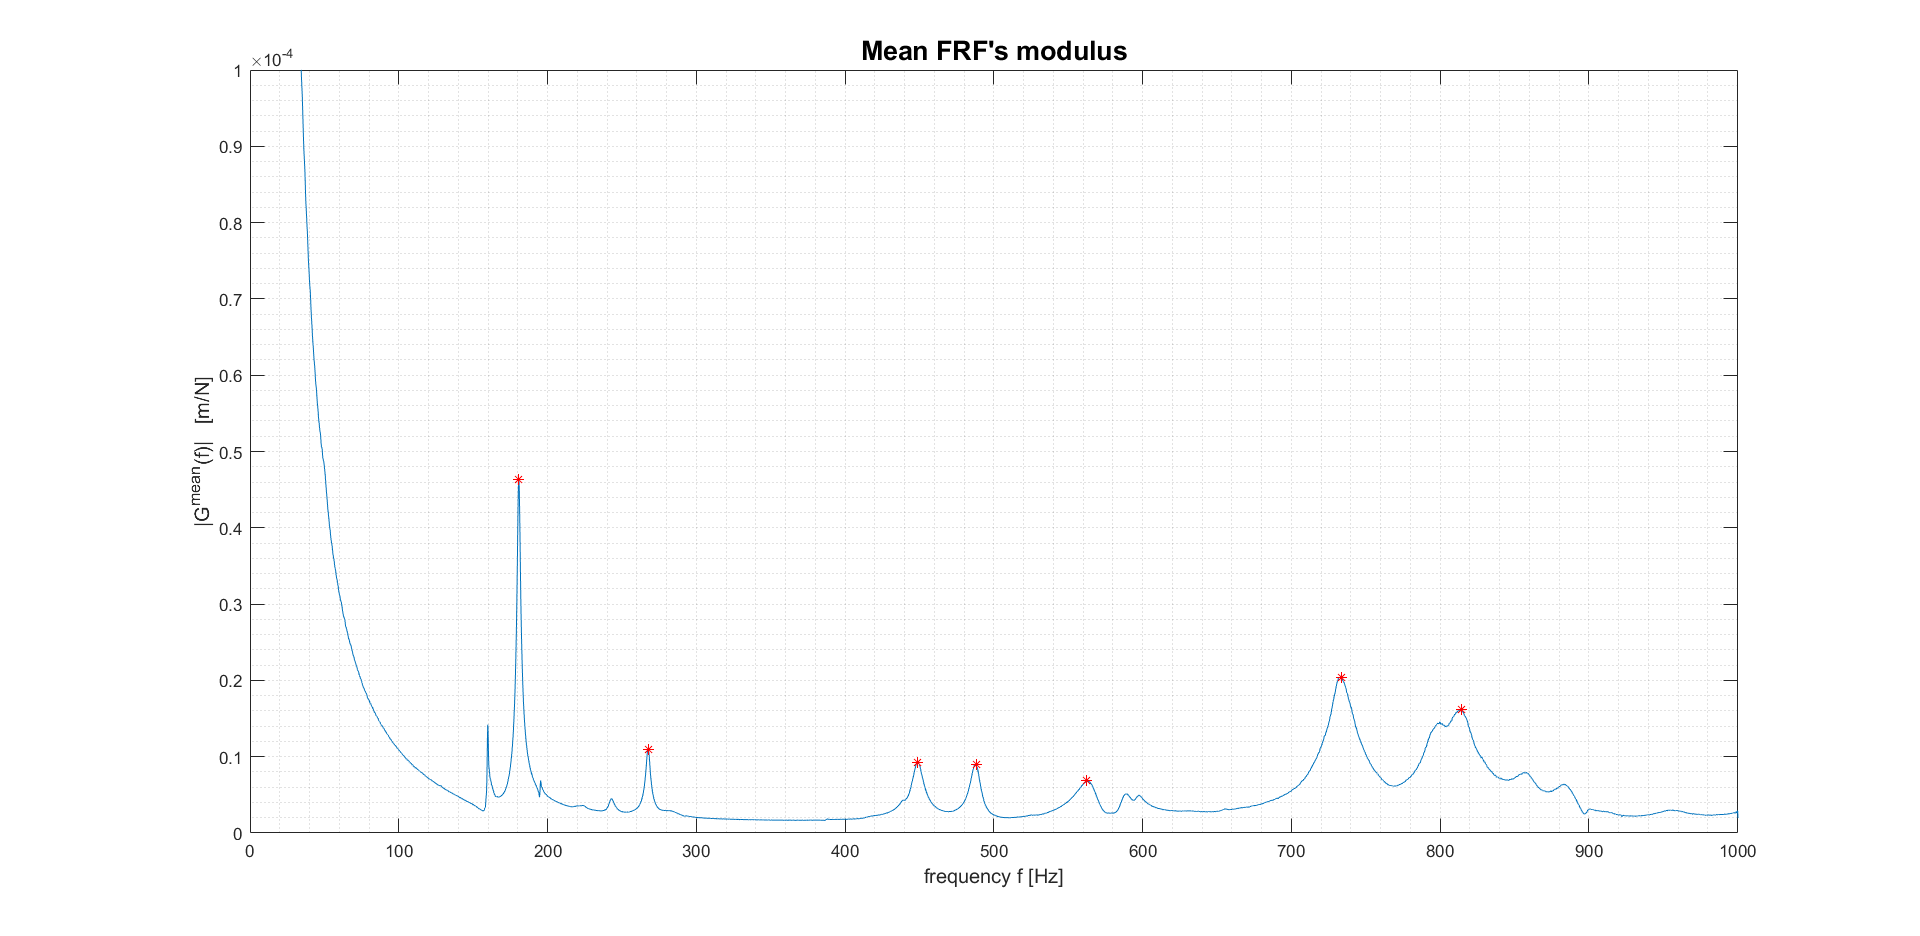
\includegraphics[scale=0.4]{frf_mean}
		\end{figure}

	\item Using \lstinline!findpeaks! to identify the most evident maxima in the mean FRF. In particular, the following snippet of code in used for searching for peaks.

		\begin{lstlisting}[caption = {Peaks' search}]
			prom = 0.000003;
			width = 8;
			tr = 0;
			iini = 500;
			[~, indices] = findpeaks(FRFmean(iini:end), 'MinPeakProminence', prom,
				'MinPeakWidth',	width, 'Threshold', tr);
			Nmodes = length(indices);
			indices = indices + iini;
		\end{lstlisting}

As it can be seen the first 500 samples are discarded in order not to consider the initial part of the FRF that diverges. This can be attributed to the structure used for holding the violin, so we're allowed to pretend the FRF starts after this region.

	\item Finding the frequency value associated with each peak. These constitute the first-guess-values for the minimization process as for the natural frequencies.

\end{itemize}

%\clearpage


\section{Results}

\subsection{Comparison between reconstructed and experimental FRFs}

Our \textsc{Matlab} script identifies 7 modes. Considering one of the 125 input-output couples, we report the reconstructed Frequency Response Function compared to the corresponding experimental one. The numerical one provides a good approximation of the original one, following its amplitude envelope. We also remind that, in case the value of the modulus for one of the identified natural frequencies is not the maximum value in the considered frequency range, we considered the actual maximum value, and its corresponding frequency, for the reconstruction of that portion of FRF. This is the case for the last peak in the showed diagram, whose frequency is $ 884 \, \text{Hz} $ in place of $ 814 \, \text{Hz} $.

\begin{figure}[H]
	\hspace{-70pt}
	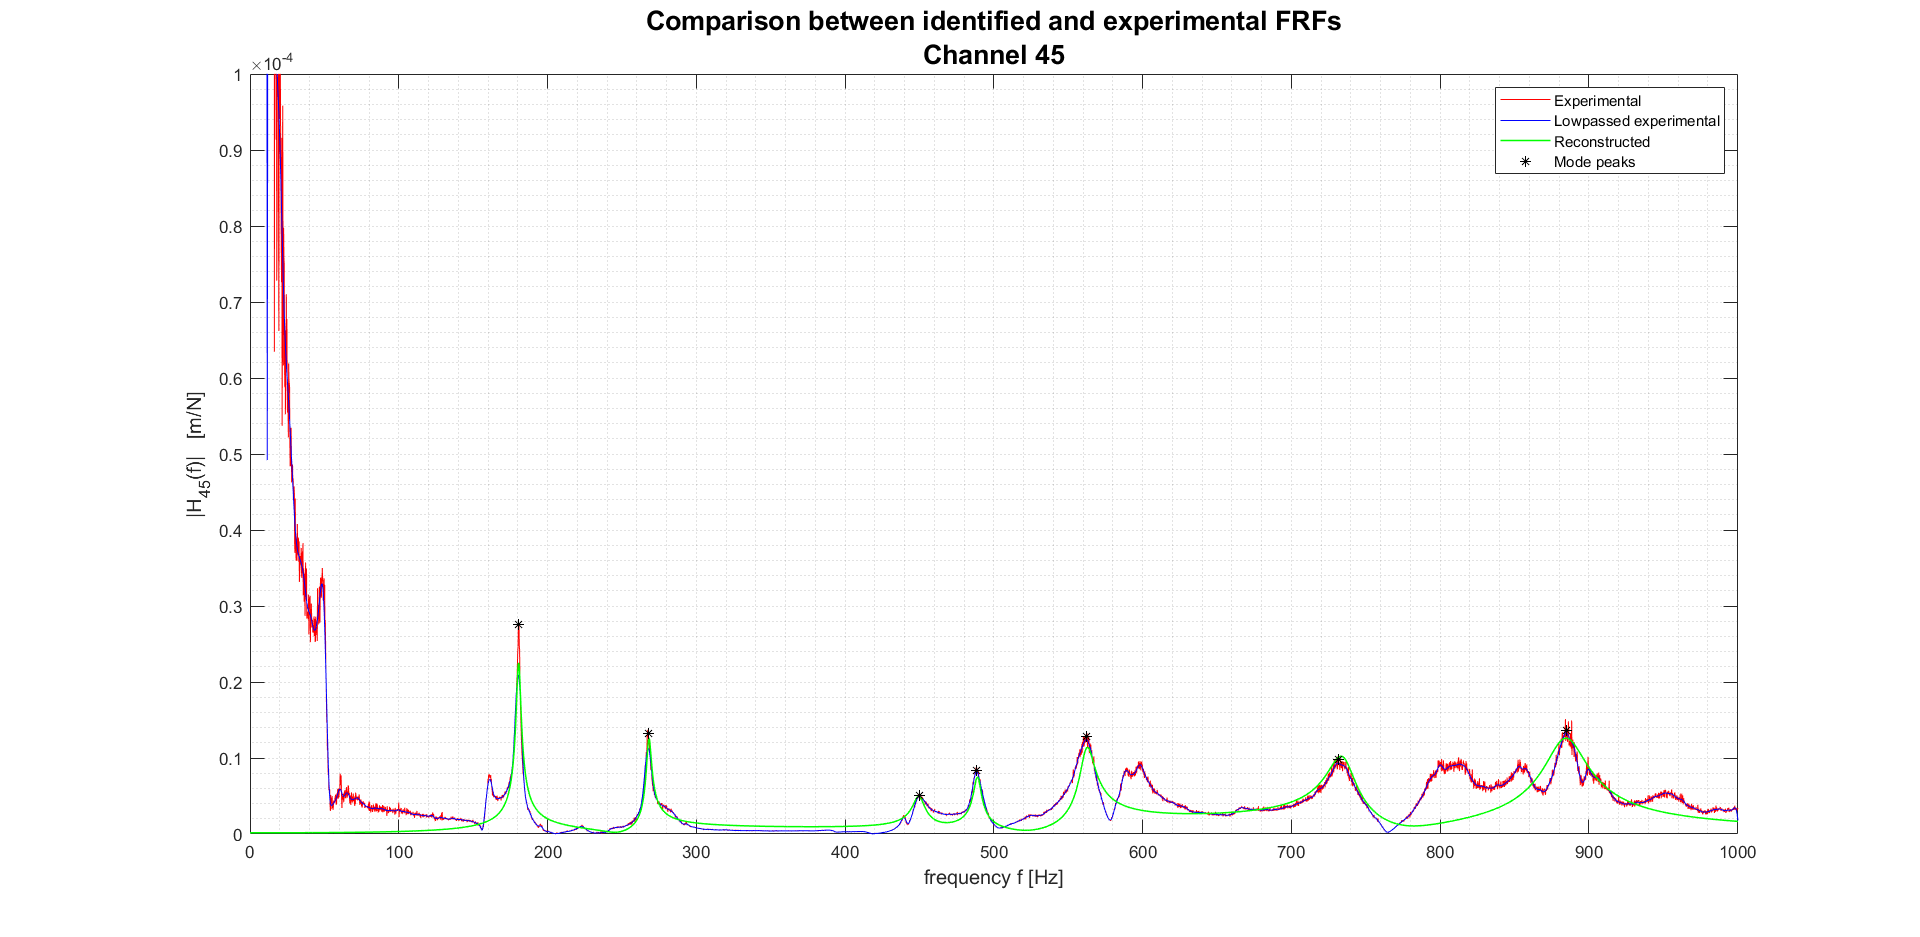
\includegraphics[scale=0.4]{frf_rec_vs_exp_ch45}
\end{figure}

Taking a closer look at some of the identified vibration modes, we may appreciate even more the fact a non-noisy FRF has been analitically obtained:

\begin{figure}[H]
	\hspace{-70pt}
	\subfloat{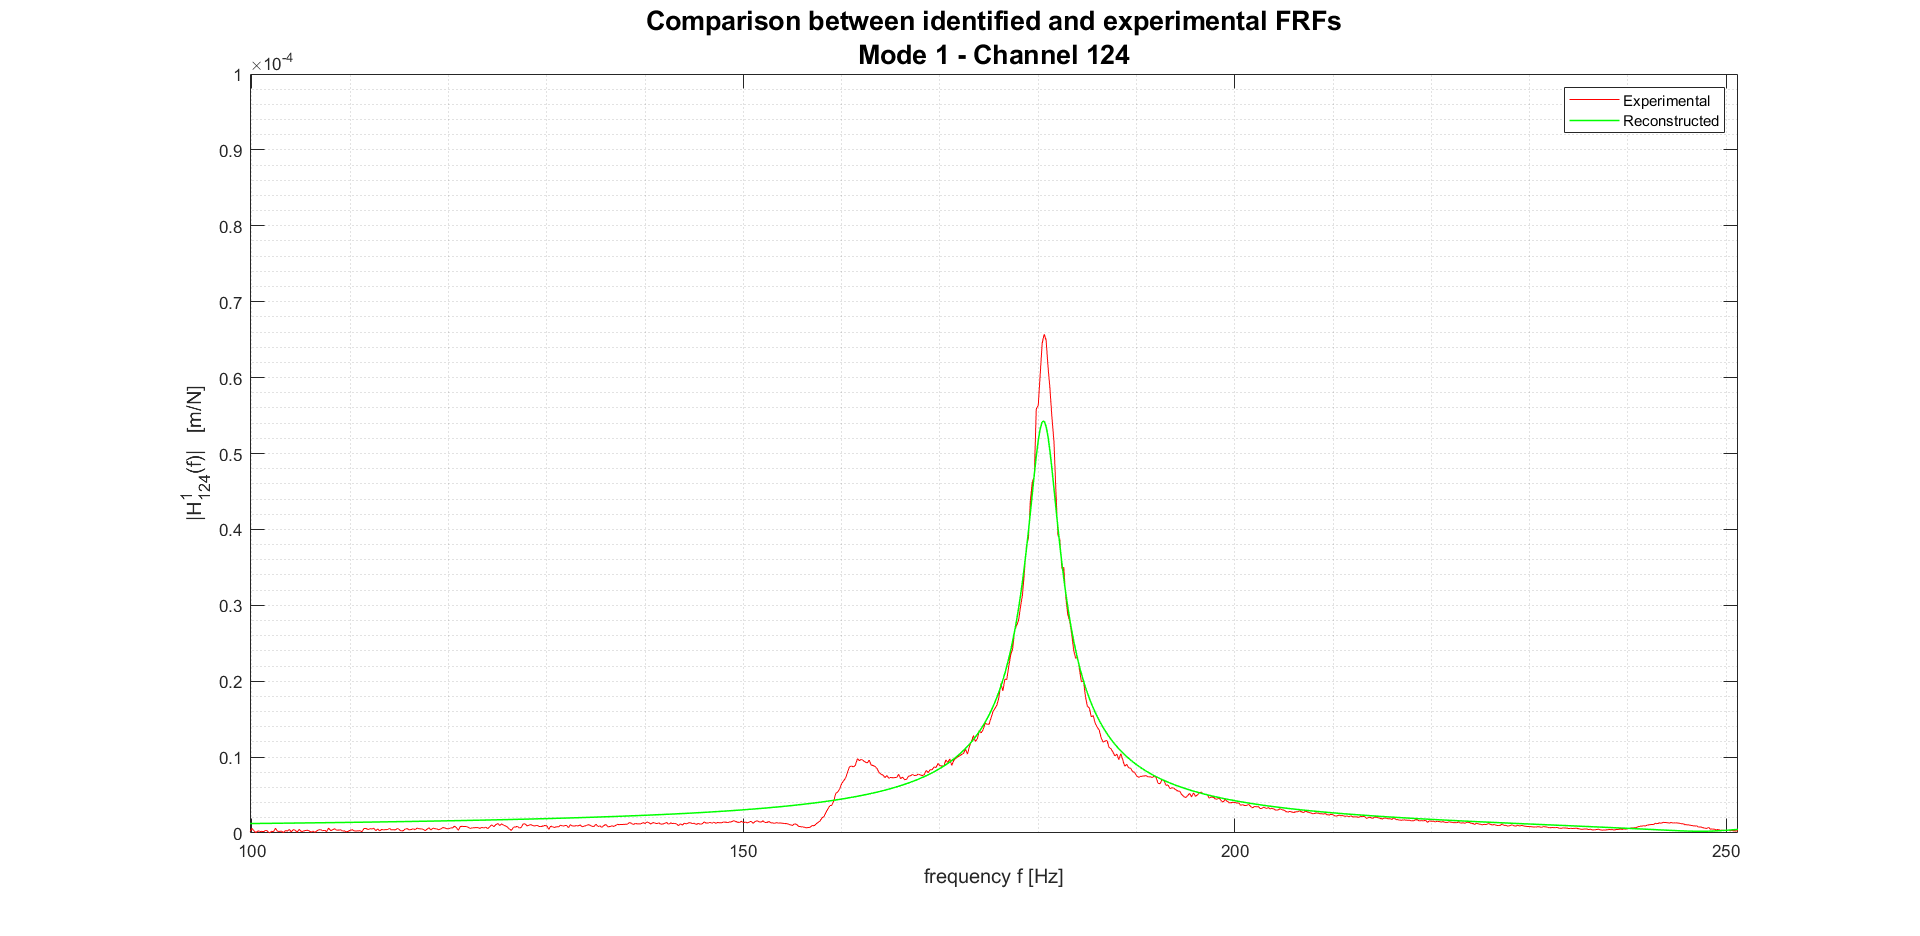
\includegraphics[scale=0.2]{frf_rec_vs_exp_mode1_channel124}}
	\subfloat{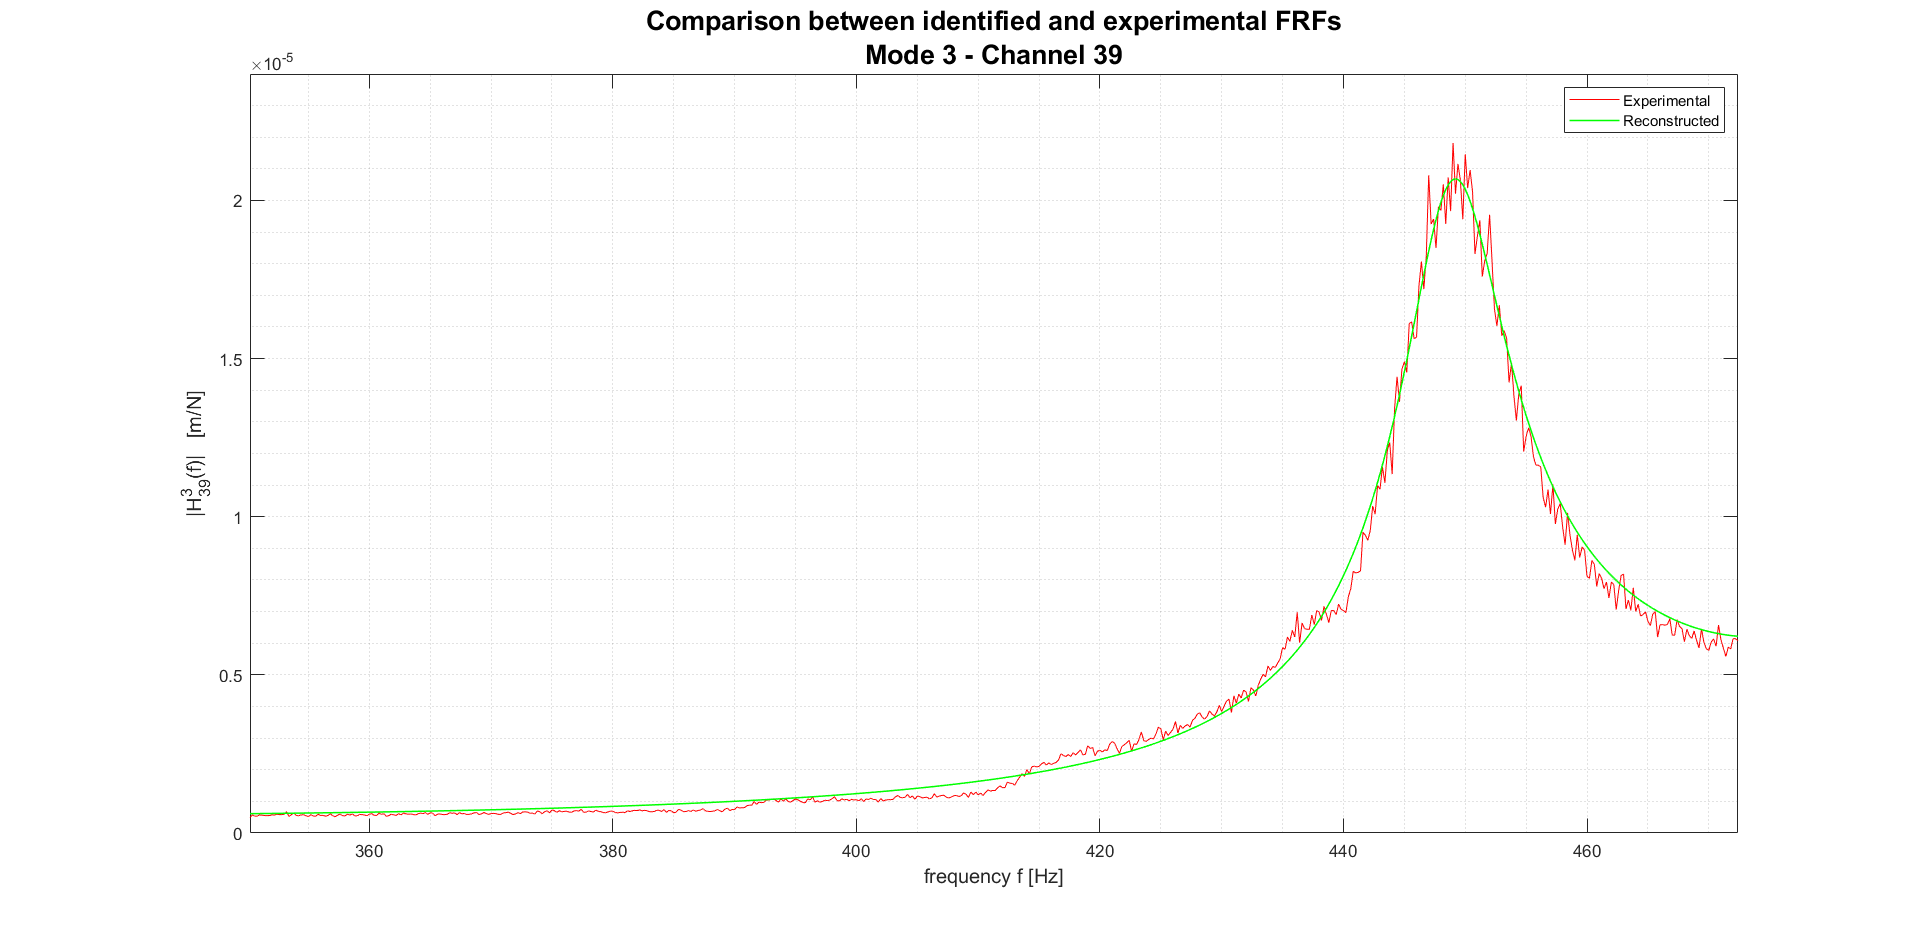
\includegraphics[scale=0.2]{frf_rec_vs_exp_mode3_channel39}}
\end{figure}
\begin{figure}[H]
	\hspace{-70pt}
	\subfloat{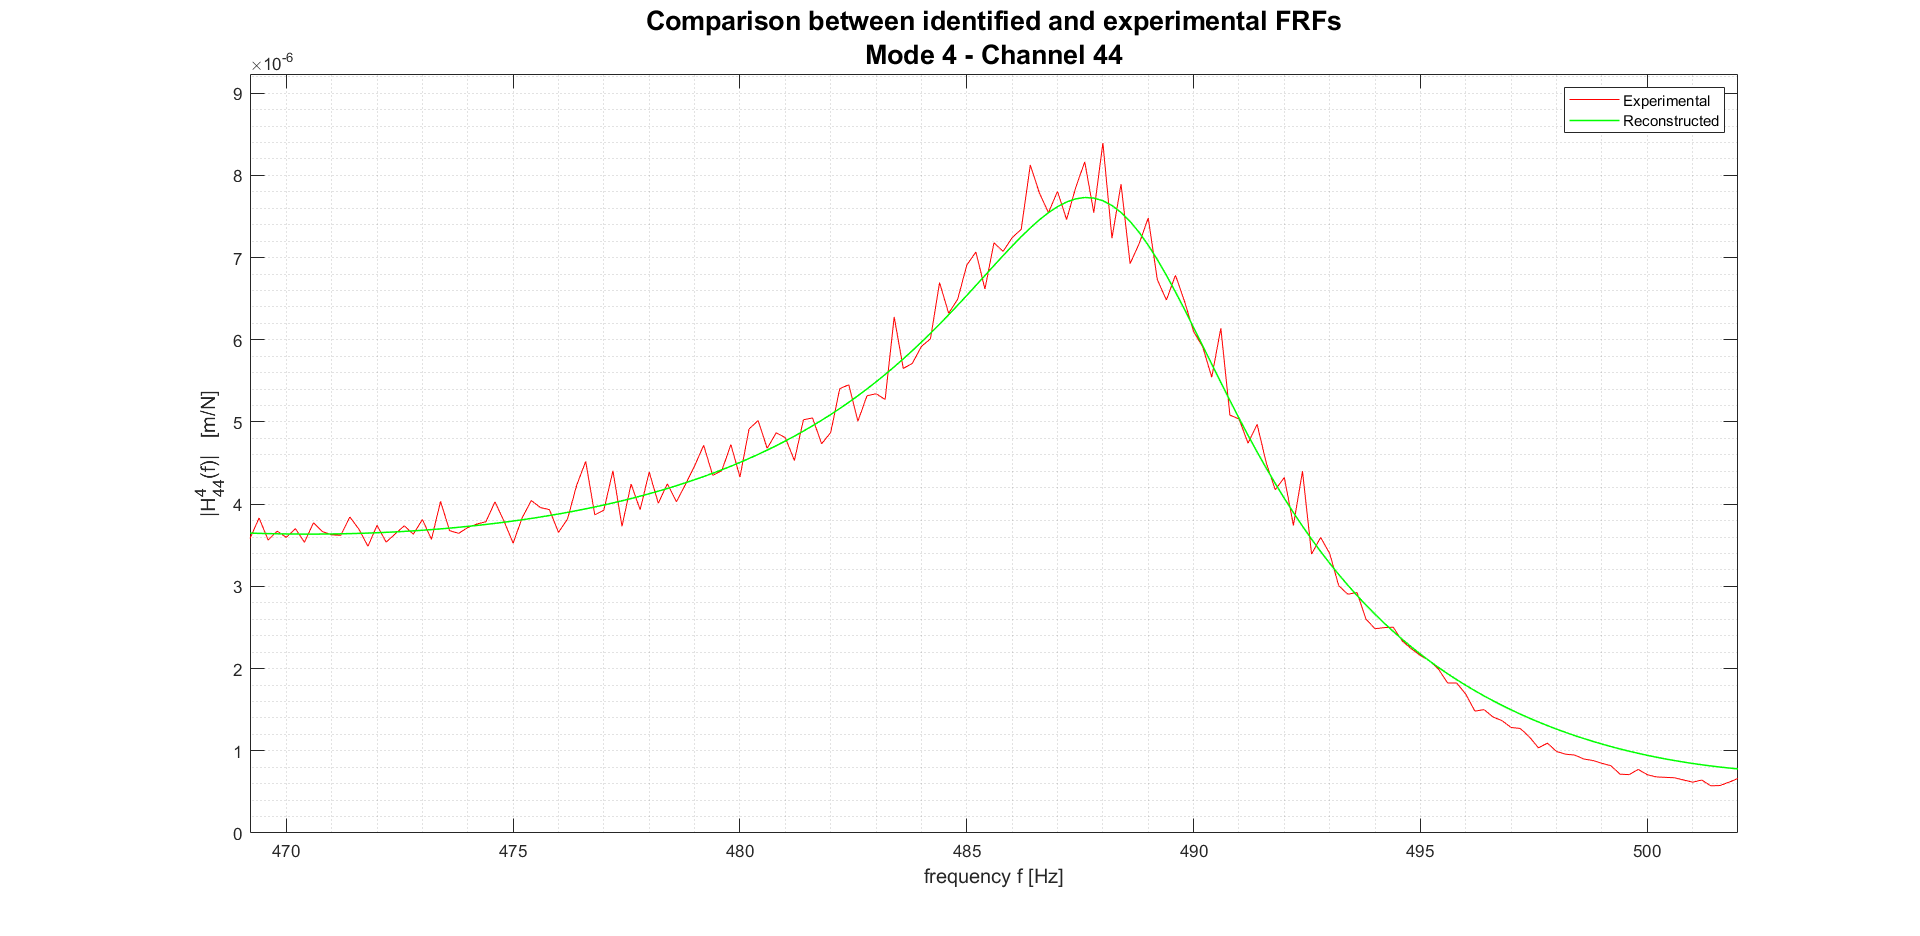
\includegraphics[scale=0.2]{frf_rec_vs_exp_mode4_channel44}}
	\subfloat{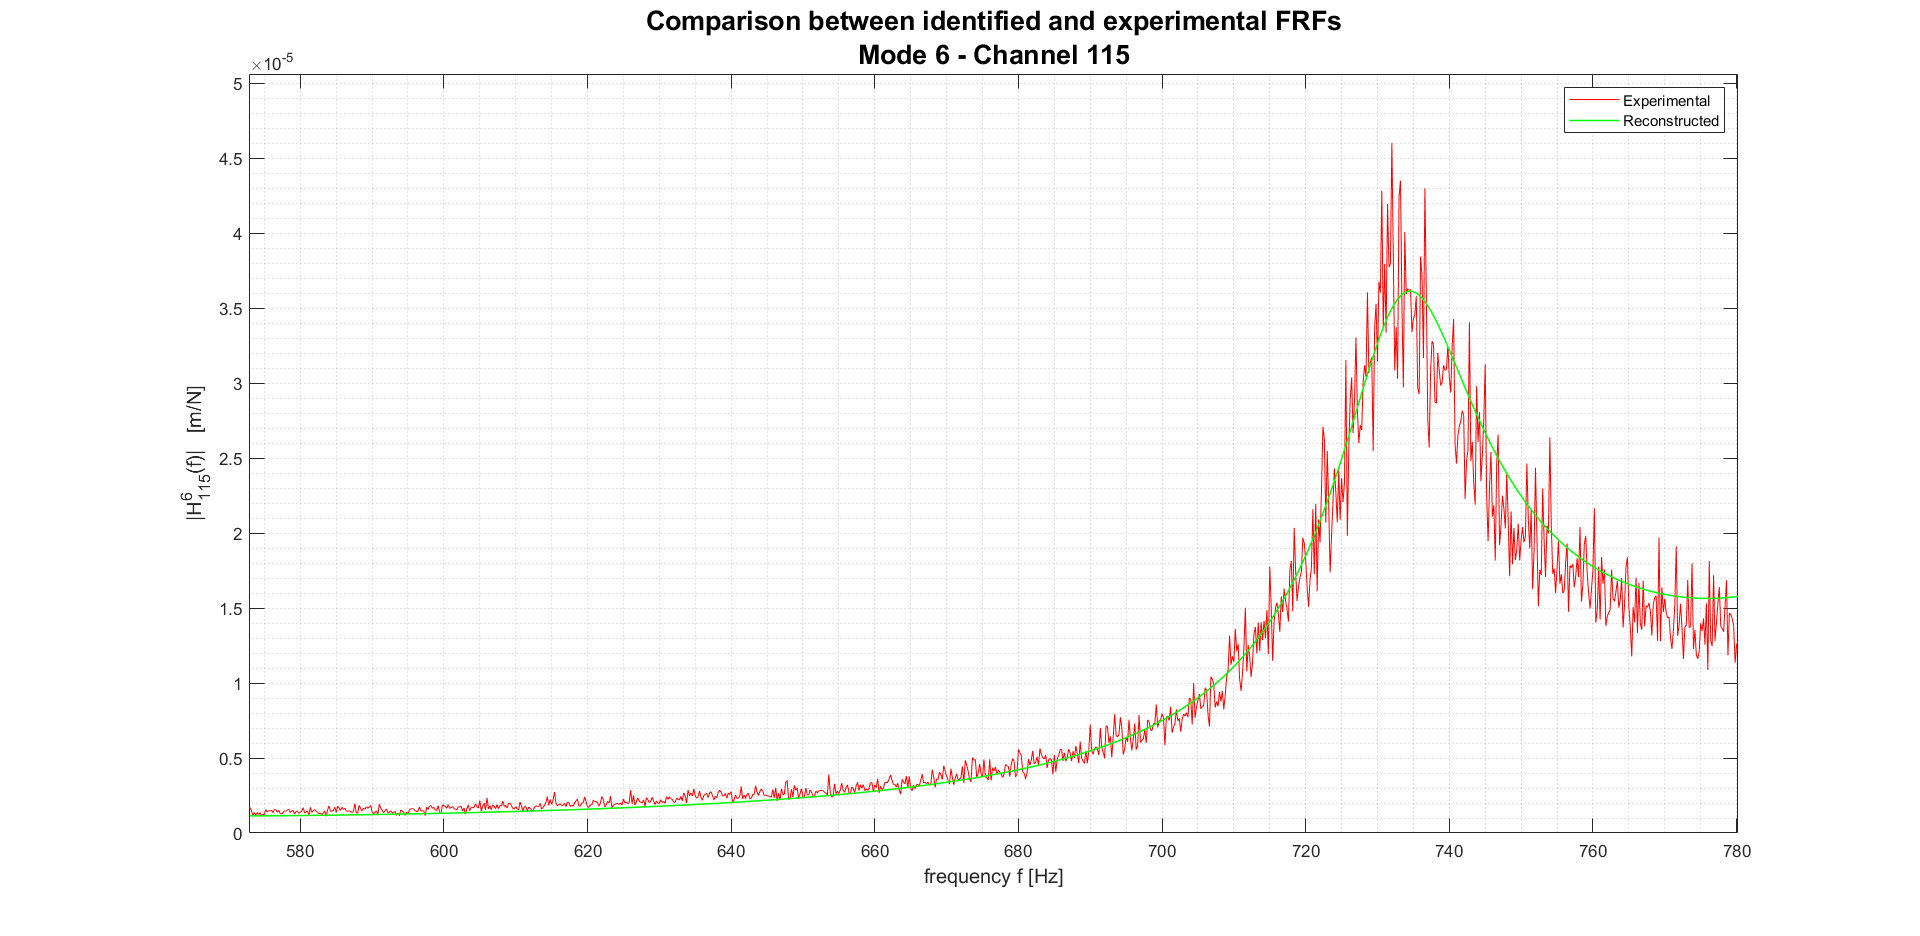
\includegraphics[scale=0.2]{frf_rec_vs_exp_mode6_channel115}}
\end{figure}

\subsection{Modal parameters}

The results in terms of natural frequencies and damping ratios for the 7 identified modes can be summarized in the following table.

\begin{table}[H]
	\centering
	\begin{tabular}{ccc}
		Mode	& Frequency {[}Hz{]}	& Damping ratio (\%) \\
		1		& 180.8						& 0.91\% \\
		2		& 267.8						& 0.78\% \\
		3		& 448.8						& 0.75\% \\
		4		& 488.2						& 0.58\% \\
		5		& 562.6						& 1.08\% \\
		6		& 733.6						& 1.22\% \\
		7		& 814.2						& 1.49\%
	\end{tabular}
\end{table}

\subsection{Identified modes}

The following plots summarize the characteristics of the vibration modes of the violin plates: for each of them, we're displaying natural frequency, adimensional damping ratio (percentage) and a graphical representation of the mode shape, indicating the displacement of the points on the surface with respect to each other for that particular oscillation mode.

\begin{figure}[H]
	\subfloat{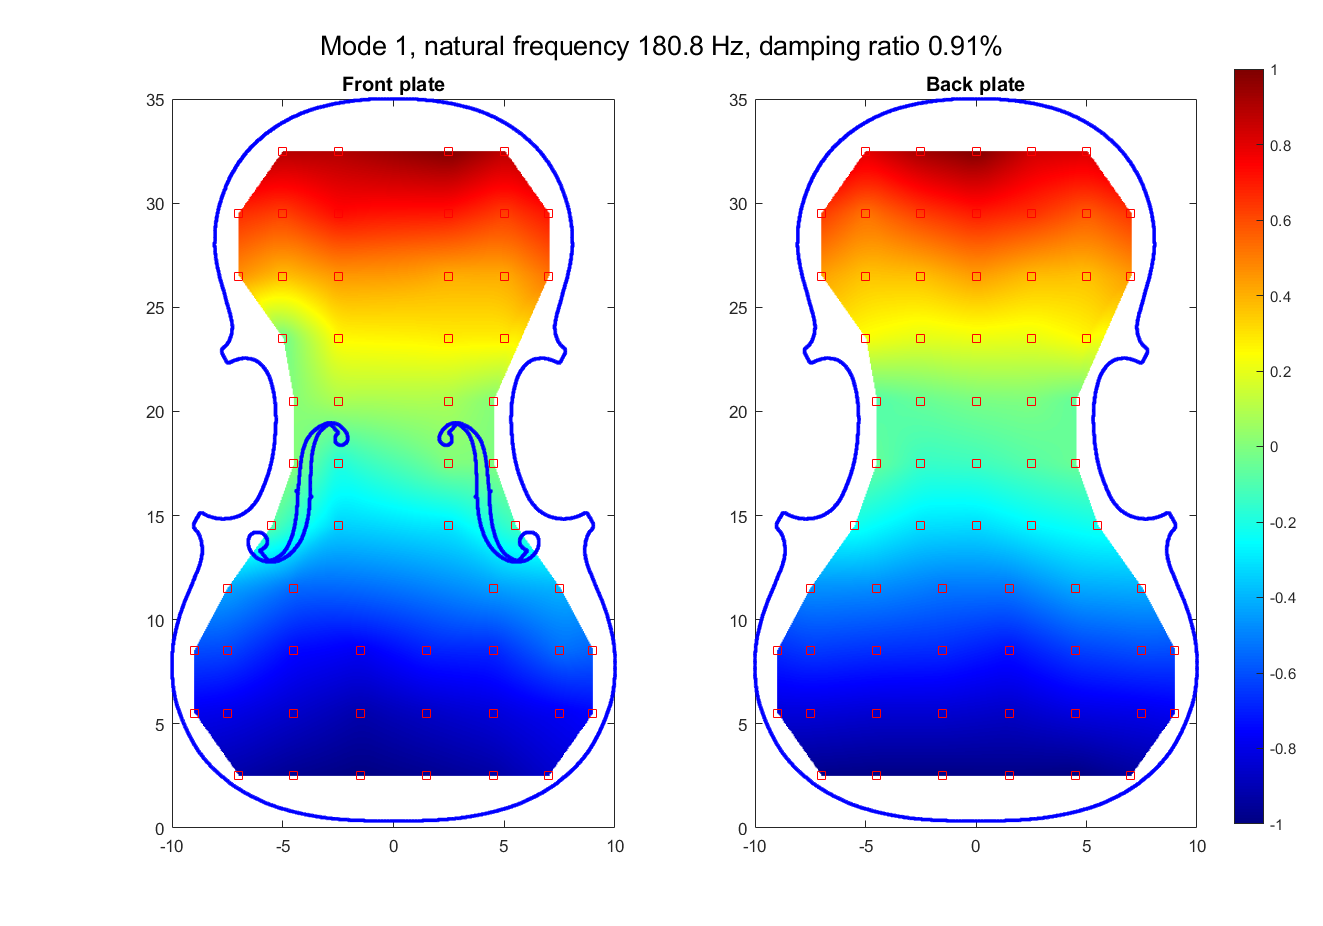
\includegraphics[scale=0.25]{violin_mode_1}} \quad
	\subfloat{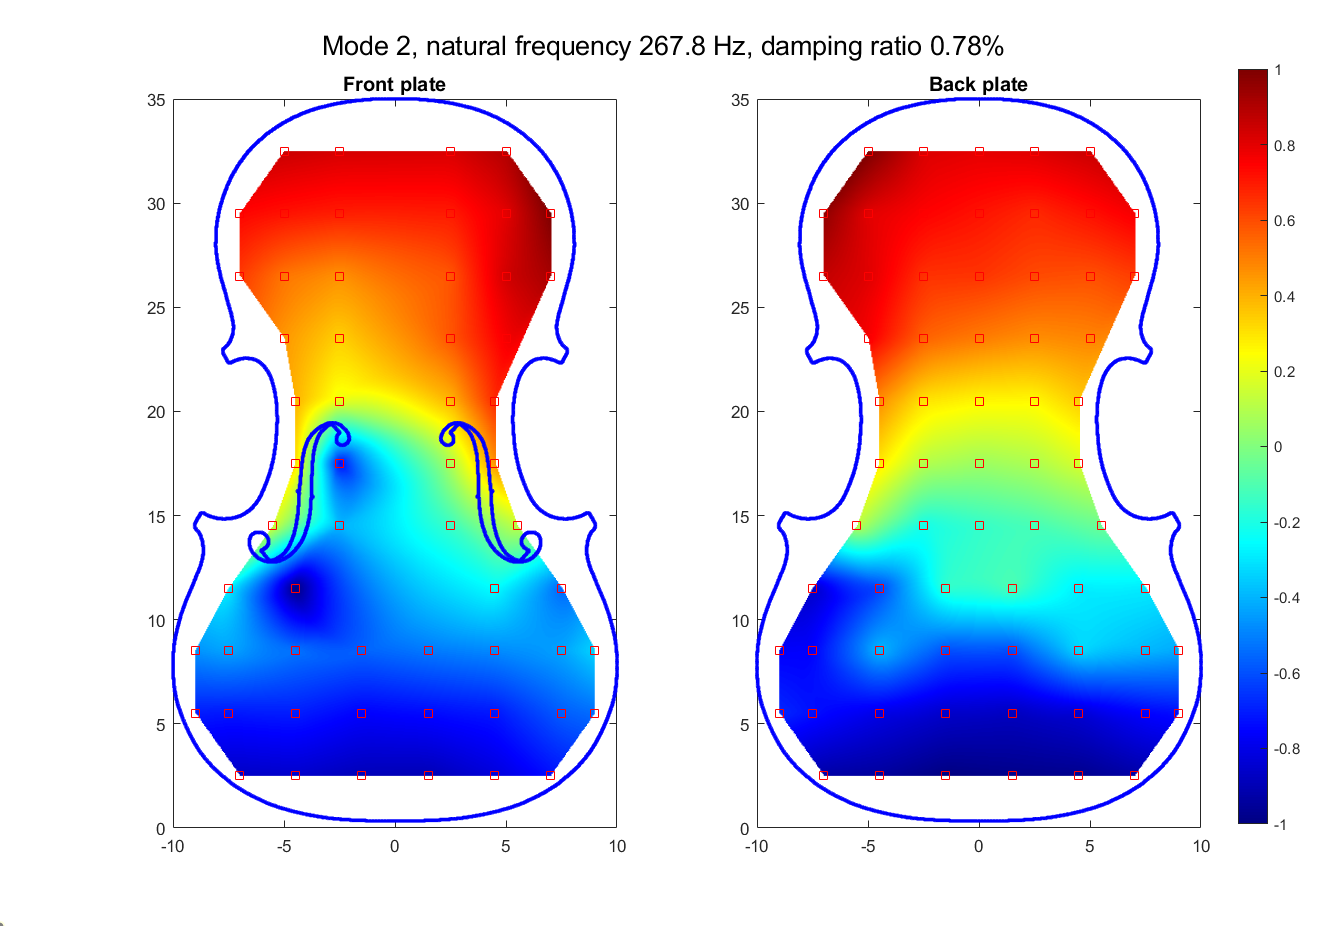
\includegraphics[scale=0.25]{violin_mode_2}} \\
	\subfloat{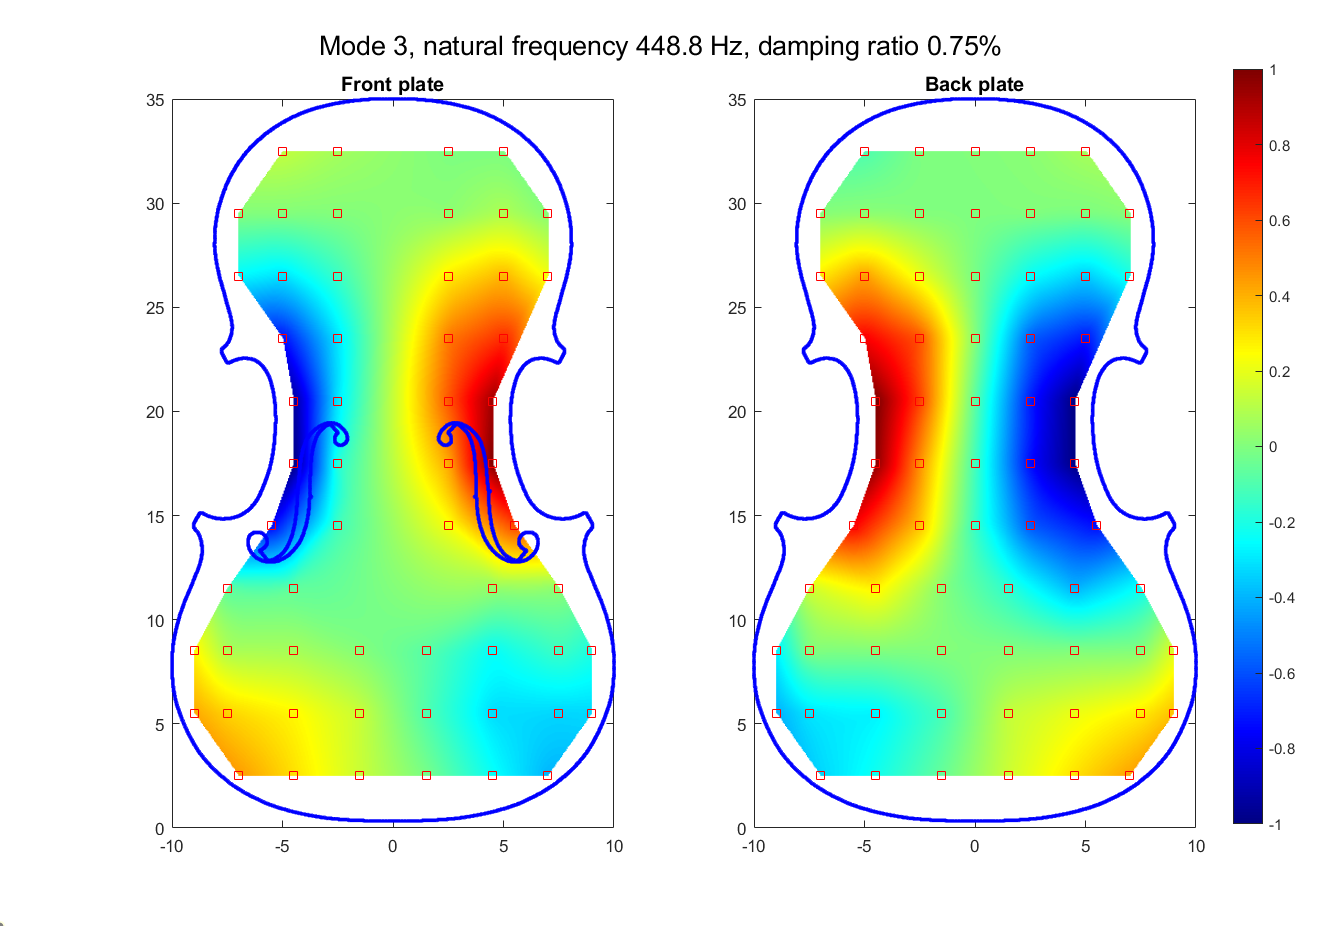
\includegraphics[scale=0.25]{violin_mode_3}} \quad
	\subfloat{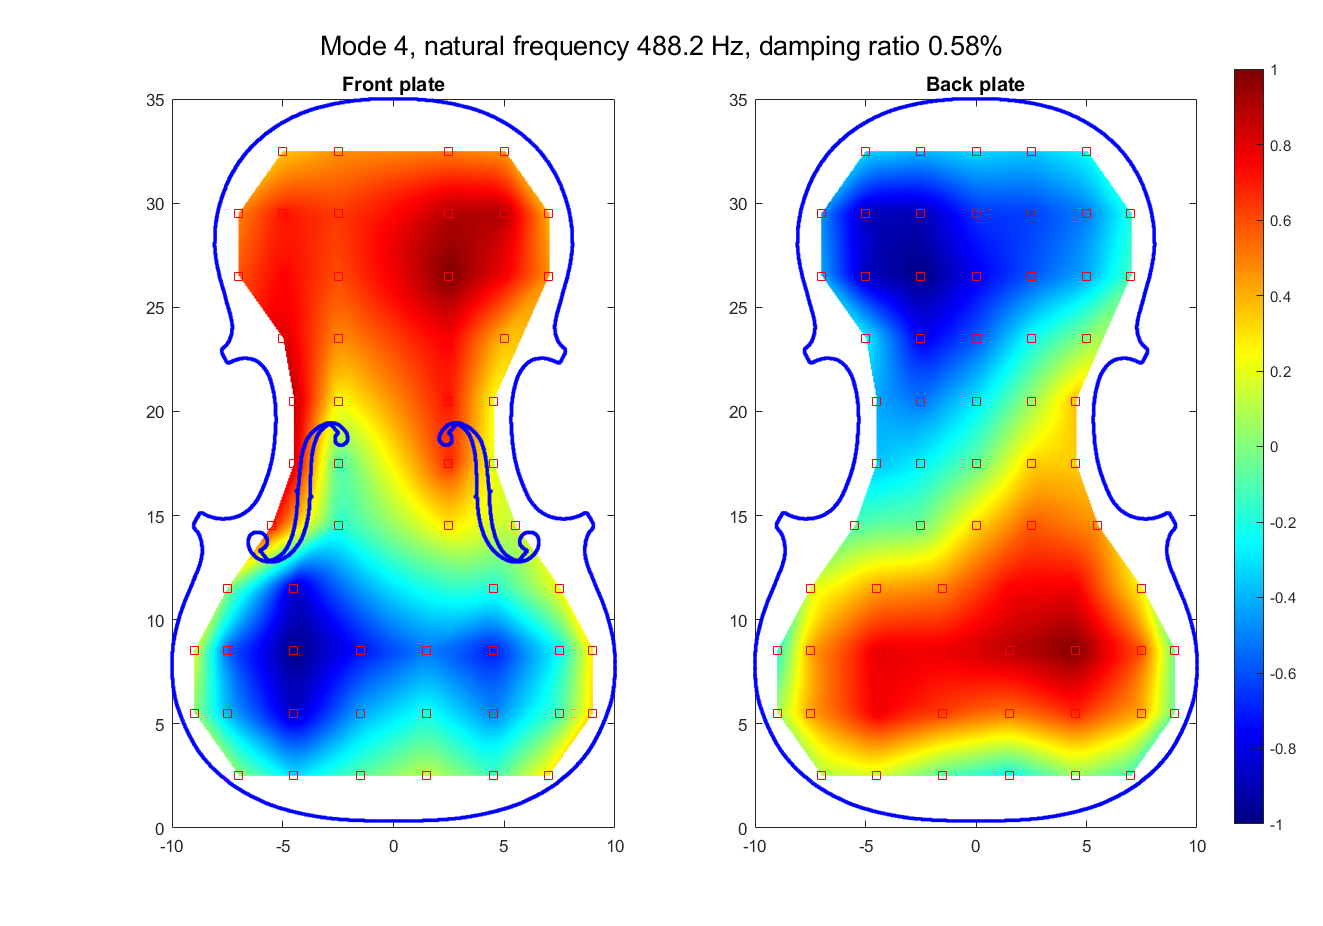
\includegraphics[scale=0.25]{violin_mode_4}} \\
\end{figure}
\begin{figure}[H]
	\subfloat{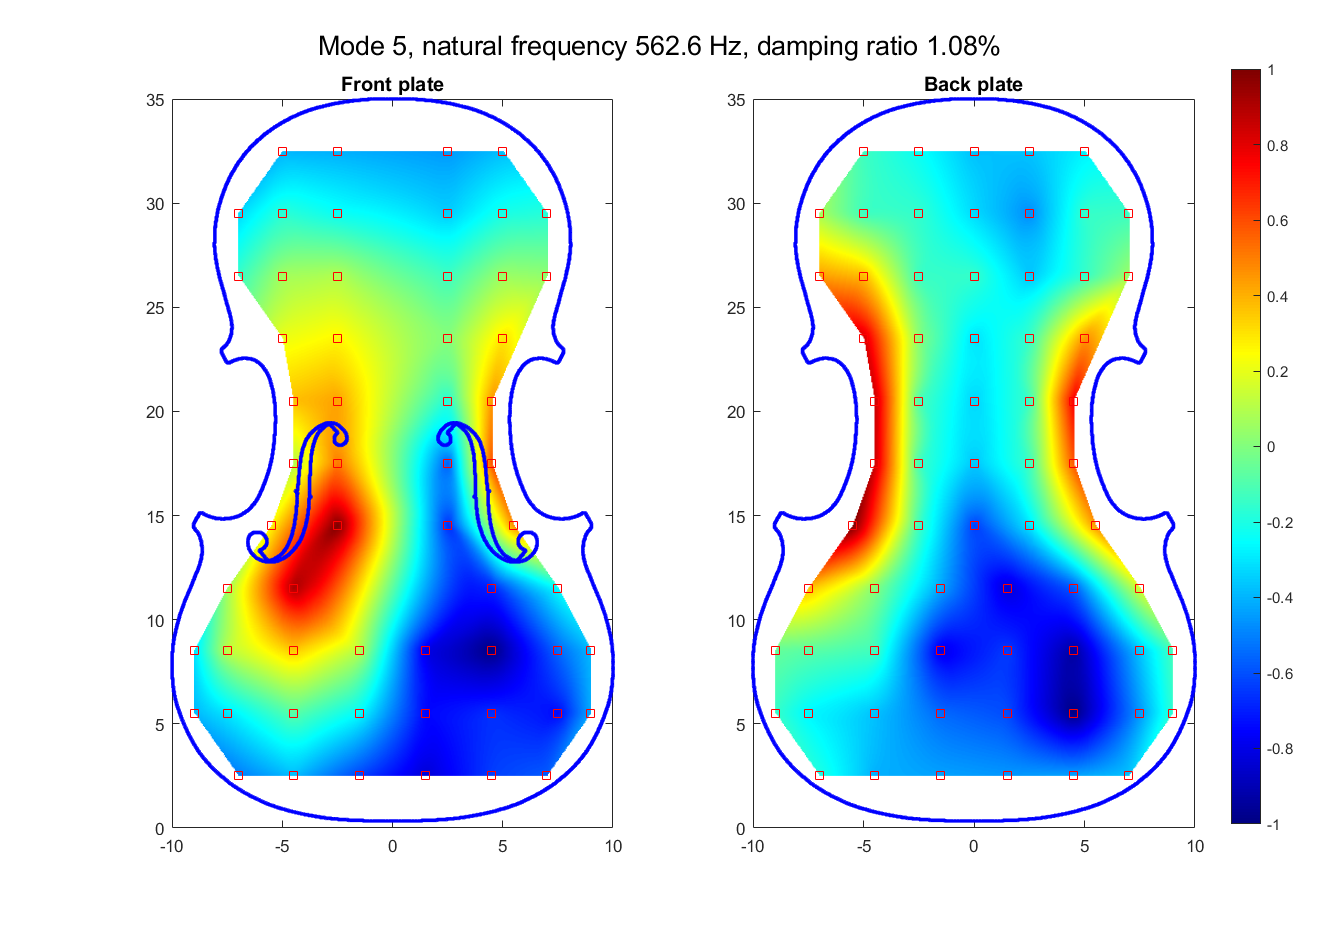
\includegraphics[scale=0.25]{violin_mode_5}} \quad
	\subfloat{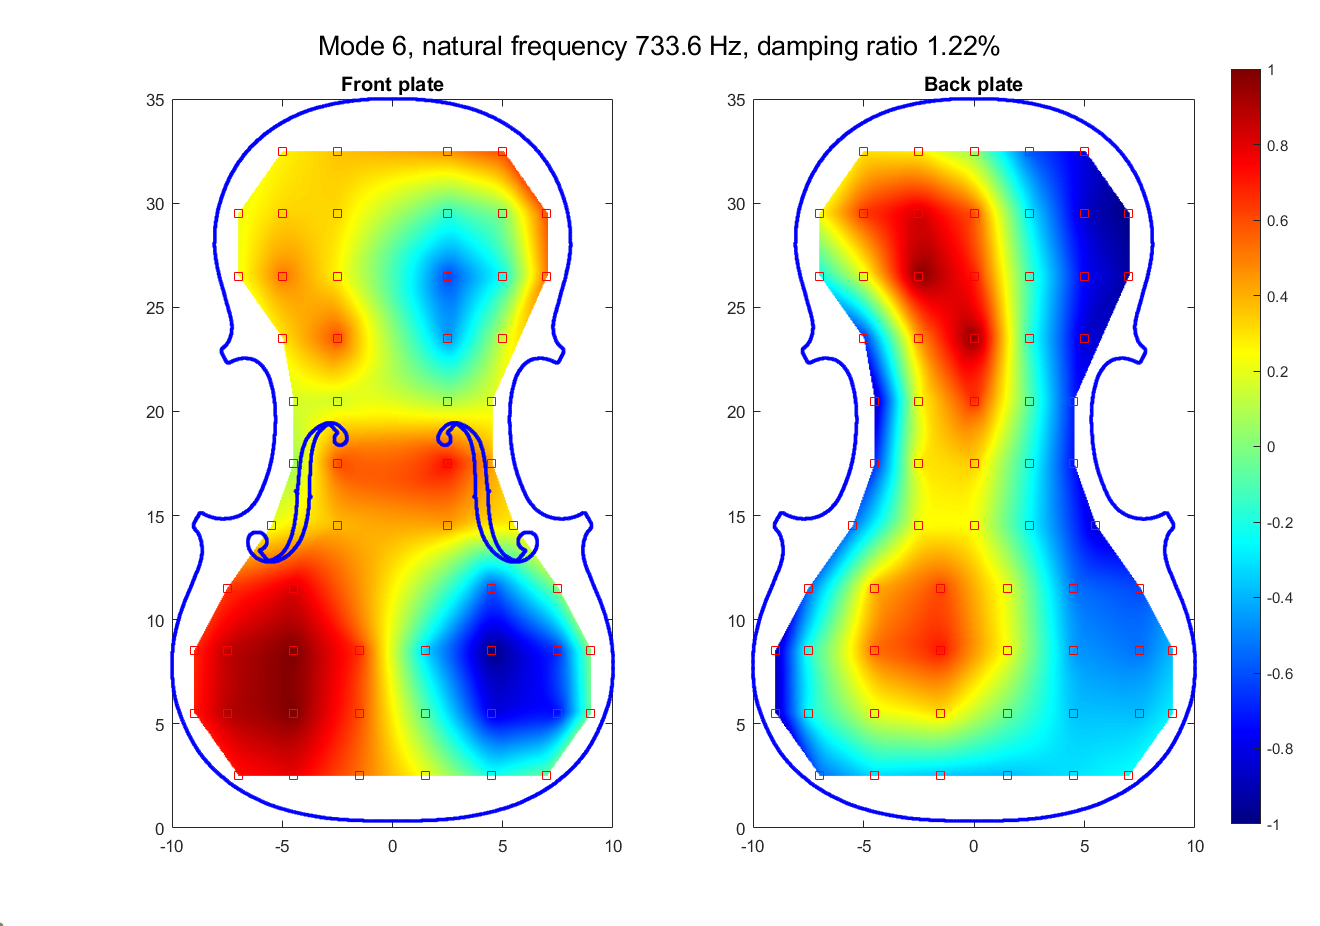
\includegraphics[scale=0.25]{violin_mode_6}} \\
	\begin{center}
		\subfloat{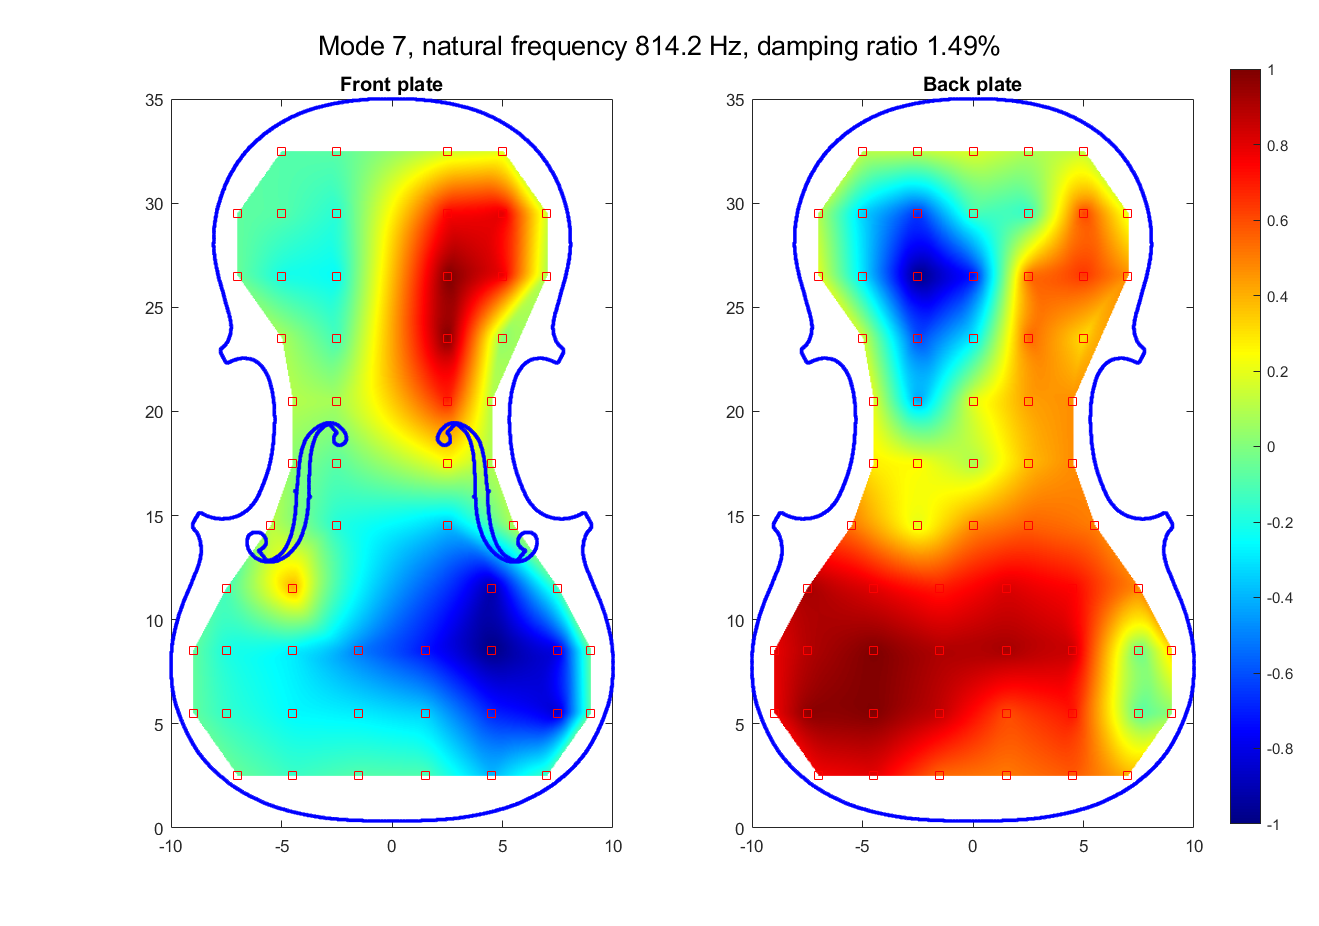
\includegraphics[scale=0.25]{violin_mode_7}}
	\end{center}
\end{figure}

As we could infer a priori, the mode shape is more and more complex as the resonating frequency increases: in the first two modes, we can easily identify two main oscillating areas (the upper part and the lower part of the plate), in accordance between top and back plate. In the third one, there are four, with crossed polarization and accordance between top and back plate, and so on. As the mode number increases, the two plates start decouple one from the other, and the oscillation modes may not correspond anymore. This is due to the fact the higher the frequencies, the more top and back plate exhibit different modes. Talking about the damping ratio, this is on average lower at lower frequencies than at higher ones.


\end{document}